\section{Decorator-Muster}

\subsection{Problemstellung}
\begin{itemize}
\item Ein B"acker m"ochte verschiedene Kaffeesorten verkaufen. 
\item Es soll m"oglich sein verschiedene Bonuszutaten (z.B. Sahne, Zucker, etc.) hinzuzuf"ugen. 
\item Hierbei kann die Menge der variieren. Es ist also m"oglich sowohl eine Extra-Portion, als auch 
  zwei extra Portionen Sahne dazu zu bestellen. 
\item Ausserdem ist es m"oglich verschiedene Zutaten zu kombinieren. 
\item Problem: Wenn man sich auf einfache Vererbung beschr"ankt wird die Stuktur sehr schnell 
  un"ubersichtlich. 
\end{itemize}

\subsection{L"osung}
Es wird zu allererst eine abstrakte Klasse Getr"ank gebildet, von der sowohl die Zutaten als auch 
die Kaffeesorten erben. Die Kaffesorten tun dies direkt. Sie besitzen zwei Felder f"ur die 
Beschreibung und den Preis, "uber entsprechende Getter sind sie abrufbar. Nun bildet man eine 
abstrakte Wrapper-Klasse von der s"amtliche Zutaten erben sollen. Jede Zutat erbt von der Wrapper 
Klasse und muss die Getter f"ur die Beschreibung / Preis neu implementieren, denn jede Zutat 
h"alt eine Referenz auf ein Getr"ank welches im Konstruktor gesetzt wird. Bei den Gettern wird 
die Beschreibung / Preis an die Werte des Getr"anks angeh"angt bzw. drauf addiert. Da alle 
Klassen von der selben Superklasse ableiten kann die Referenz nicht nur einen Kaffee ohne Zutaten 
sondern auch einen mit diesen beinhalten. Die Wrapper-Klasse ist letztendlich dazu da eine 
Schnittstelle herzustellen, damit es sowohl geordnet ist und die Referenz wie erw"ahnt 
bereits modifizierte Objekte halten kann. 

Beim Bestellen wird eine zugrunde liegende Kaffesorte gew"ahlt (z.B. Espresso). Diese wird mit 
den einzelnen Zutaten "dekoriert" (Bsp. siehe main Klasse im Code). 

\subsection{Erkl"arung des Musters}
\paragraph{Definition}
Decorator - F"ugt einem Objekt dynamisch zus"atzliche Verantwortlichkeit hinzu. Dekorierer bieten 
eine flexible Alterntive zur Ableitung von Unterklassen zum Zweck der Erweiterung der 
Funktionalit"at.

\paragraph{Punkt f"ur Punkt (S.105)}
\begin{itemize}
\item Vererbung ist eine Form von Erweiterung, aber nicht notwendigerweise der beste Weg, um Ihren 
  Entw"urfen Flexiblit"at zu verleihen. 
\item Unsere Entw"urfe sollen die Erweiterung von Verhalten ermoeglichen, ohna dass dazu bestehnder 
  Code ge"andert werden m"usste.
\item Oft keonnen Komposition und Delegierung verwendet werden, um zur Laufzeit neue Verhalten 
  hinzuzuf"ugen.
\item F"ur die Erweiterung von Verhalten bietet das Decorator-Muster eine Alternative zur Ableitung 
  von Unterklassen.
\item Das Decorator-Muster schliesst einen Satz von Dekorierer-Klassen ein, die verwendet werden, um 
  konkrete Komponenten einzupacken. 
\item Dekorierer-Klassen spiegeln den Typ der Komponente wider, die sie dekorieren. (Sie haben sogar 
  tats"achlich den gleichen Typ wie die Komponente, die sie dekorieren, entweder durch Vererbung 
  oder durch die Implementerung eines Interface.)
\item Dekorierer "andern das Verhalten der Komponenten, indem sie vor und / oder nach (oder auch an 
  Stellen von) Methodenaufrufen auf der Komponente neue Funktionalit"aten hinzuf"ugen. 
\item Sie koennen eine Komponente mit einer bliebigen Zahl vn Dekorierern einpacken. 
\item Dekorierer sind f"ur die Clients der Komponente "ublichweise transparent, ausser wenn sich der 
  Client auf den konkreten Typ der Komponente st"utzt.
\item Dekorierer koennen in Ihren Entw"urfen zu vielen kleinen Objekten f"urhen, und eine 
  "uberm"assige Verwendung kann den un"ubersichtlich machen.  
\end{itemize}
 
\paragraph{Wann das Decorator-Muster ungeeignet ist}
\begin{itemize}
\item Wenn Sie mit Code arbeiten, der auf den Typ einer konkreten Komponente angewiesen ist, 
  zerbrechen Dekorierer diesen Code. Solange Sie nur Code auf Basis des abstrakten 
  Komponententyps schreiben, bleibt die Verwendung von Dekorierern f"ur ihren Code transparent.
  (Muster z.B. f"ur Rabatsystem beim Kaffeehaus aus diesem Kapitel ungeeignet.)
\item Dekorierer sollen den Objekten, die sie einpacken Verhalten hinzuf"ugen. Wenn Sie begninnen, 
  auf mehreren Schichten in der Dekoriererkette zu blicken, dann strecken Sie Decorator "uber 
  seinen eigentlichen Zweck.
\end{itemize}
  
\paragraph{Gut zu wissen}
\begin{itemize}
\item Die java.io-Klassen verwenden ebenfalls das Decorator-Muster. Es gibt diverse Streams mit 
  jeweils unterschiedlichen Aufgaben, und es gibt die Klasse FilterInputStream die als Superklasse 
  f"ur verschiedene Dekorierer arbeitet.
\end{itemize}

\begin{figure}
	\centering
	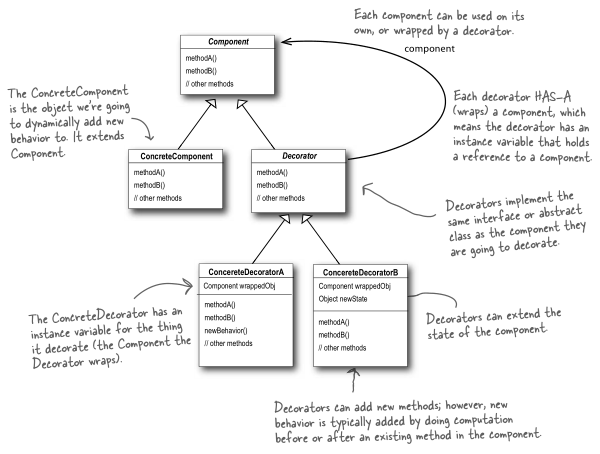
\includegraphics{decorator/img/decoratorUML}
	\caption{UML-Darstellung des Decorator-Musters}
	\label{fig:decoratorUML}
\end{figure}
